\clearpage
\section{Trajectory planning}
\subsection{Point to point tracking}
The manipulator is most likely to follow a path so it is desirable to test the controller for a path as well. The \figref{fig:pathTS} shows how each joint manages to follow the desired path used in Chapter \ref{chap:kinematics} shown in \figref{fig:IKcom} . One can see that the robot lags behind the desired path. This path is only time dependent so it changes without respect to if the robot arm has managed to get the desired position or not.\\\\
\def\picsSiz{1.08}
\begin{figure*}[htbp]
    \centering
    \begin{subfigure}[htbp]{0.45\textwidth}
        \centering
        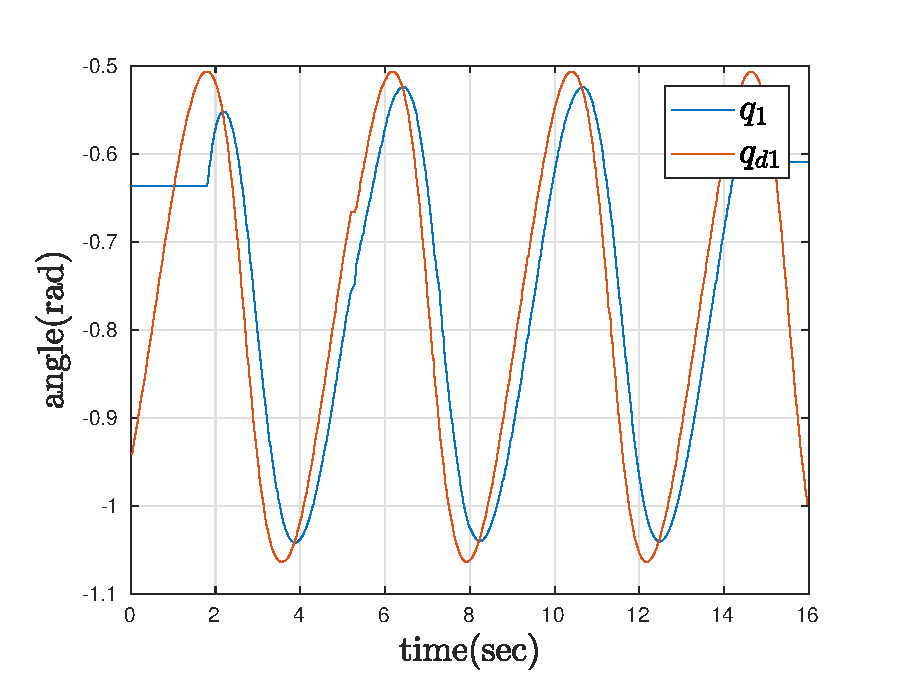
\includegraphics[width = \picsSiz\linewidth]{img/pathF1.eps}
        \caption{}
    \end{subfigure}
    ~ 
    \begin{subfigure}[htbp]{0.45\textwidth}
        \centering
        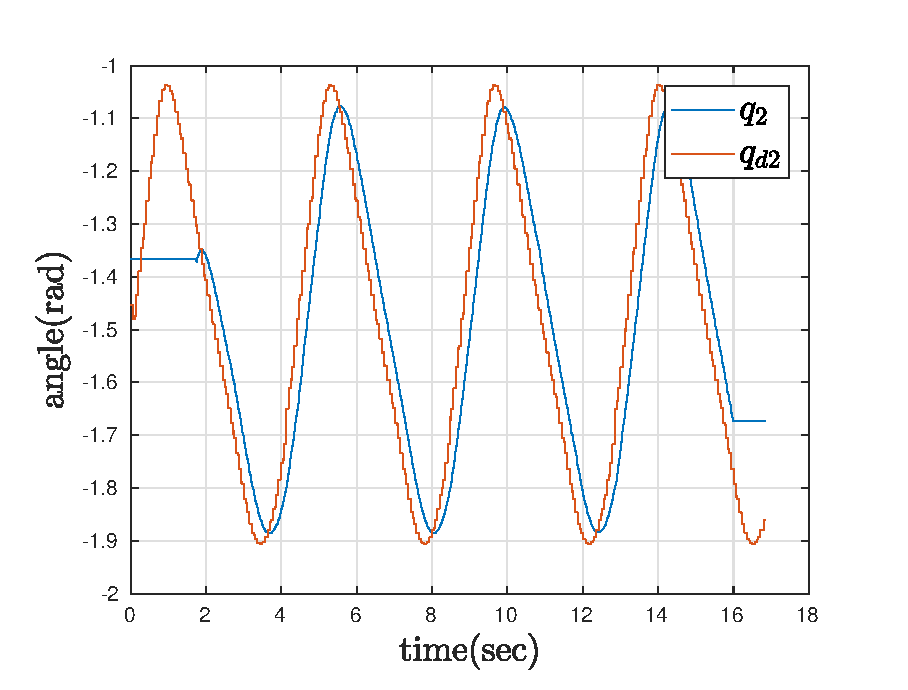
\includegraphics[width = \picsSiz\linewidth]{img/pathF2.eps}
        \caption{}
    \end{subfigure}
    ~
    \centering
    \begin{subfigure}[htbp]{0.45\textwidth}
        \centering
        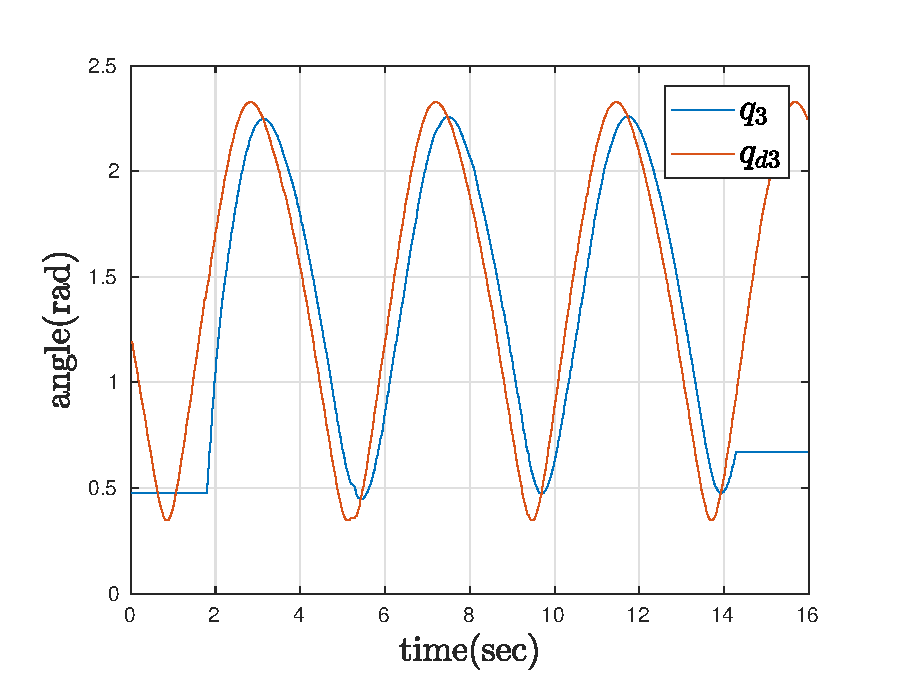
\includegraphics[width = \picsSiz\linewidth]{img/pathF3.eps}
        \caption{}
    \end{subfigure}
    ~ 
    \begin{subfigure}[htbp]{0.45\textwidth}
        \centering
        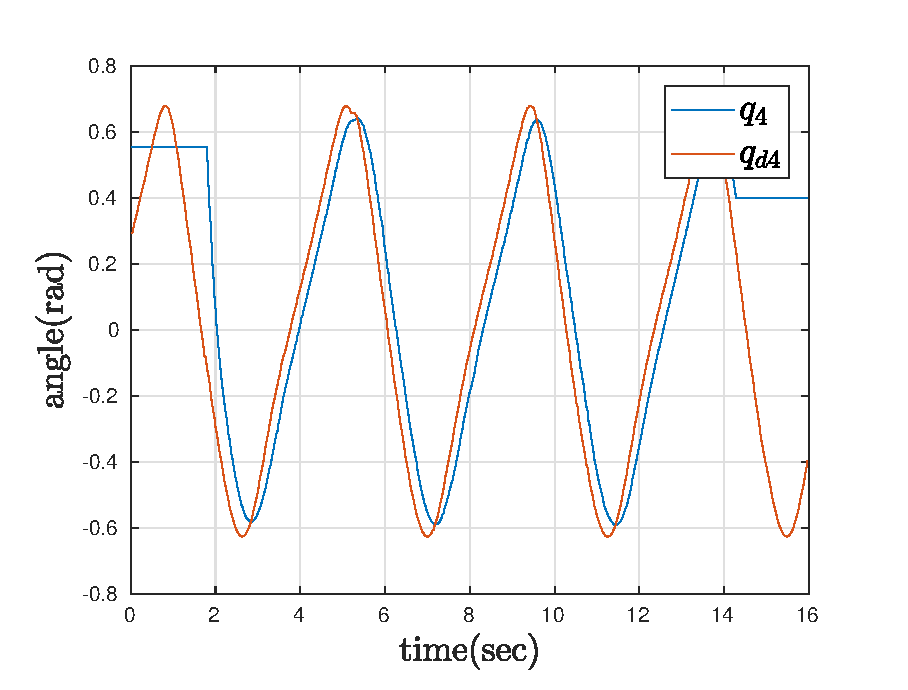
\includegraphics[width = \picsSiz\linewidth]{img/pathF4.eps}
        \caption{}
    \end{subfigure}
    ~
    \begin{subfigure}[htbp]{0.45\textwidth}
        \centering
        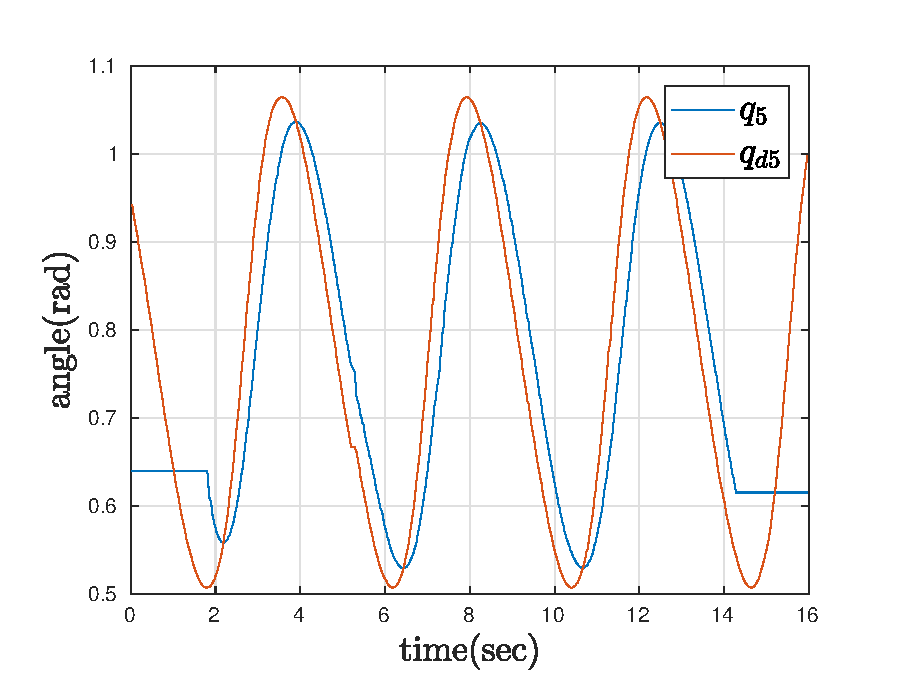
\includegraphics[width = \picsSiz\linewidth]{img/pathF5.eps}
        \caption{}
    \end{subfigure}
    \caption{Path following}
    \label{fig:pathTS}
\end{figure*}
The only information the robot gets is the point it is supposed to get to and it changes before it can reach it. It is therefore wanted to pass it some more information about the path. Reference \cite{Siciliano} gives a method to use the slope of the trajectory to find the joint velocity in the trajectory:
\begin{align*}
    \dot{q}_{d_i} = 
    \begin{cases}
    0\hphantom{ \frac{1}{2}(v_i+v_{i+1})}\;\;sgn(v_k)\ne sgn(v_{i+1})\\
    \frac{1}{2}(v_i+v_{i+1}) \quad  sgn(v_i)= sgn(v_{i+1})
    \end{cases}
\end{align*}
where $v_i = \frac{q_i-q_{i-1}}{t_i-t_{i-1}}$ and when the last point $N$ is reached, the joint velocity $q_N$ should be zero. Since the error between the executed trajectory and the desired trajectory can be seen as a time delay one can also add the next points as a reference:
\begin{align*}
    \tilde{q} = q_{d_i}-q + \frac{q_{d_{i+1}}-q }{2}+\frac{q_{d_{i+2}}-q }{2}
\end{align*}
The results are given in \figref{fig:pathTSff}. One can see that the error is almost gone. The reason integral action is not used here is because integral action is best when dealing with steady state constant errors which is not the case here\footnote{The gravity component in the controller acts as integral action by cancelling the gravity forces influencing the manipulator}. Integral action will also include more oscillations and instability to the system which is undesirable.



\def\picsSiz{1.08}
\begin{figure*}[htbp]
    \centering
    \begin{subfigure}[htbp]{0.45\textwidth}
        \centering
        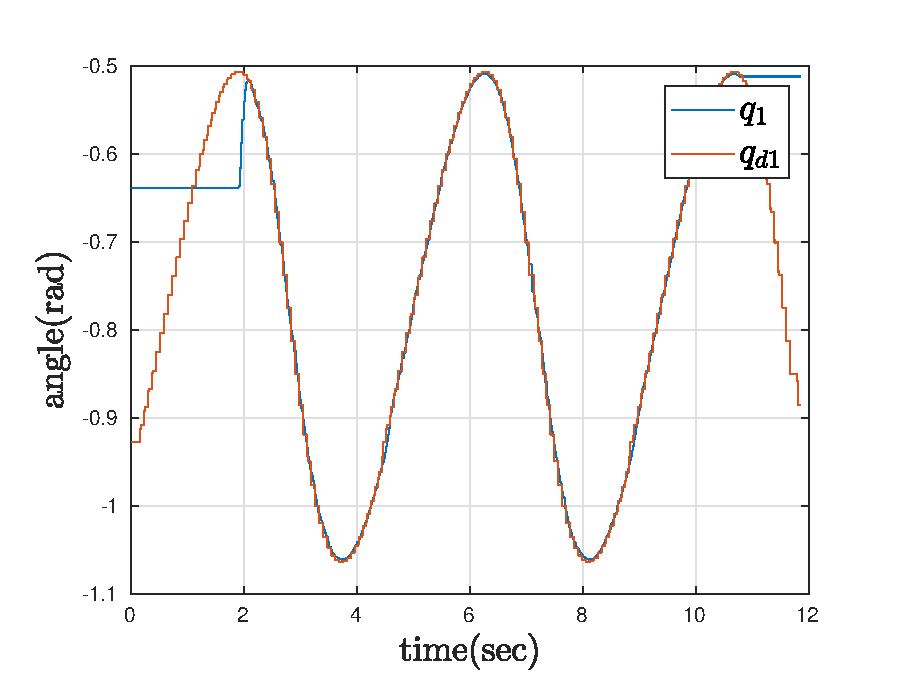
\includegraphics[width = \picsSiz\linewidth]{img/pathF1ff.eps}
        \caption{ }
    \end{subfigure}
    ~ 
    \begin{subfigure}[htbp]{0.45\textwidth}
        \centering
        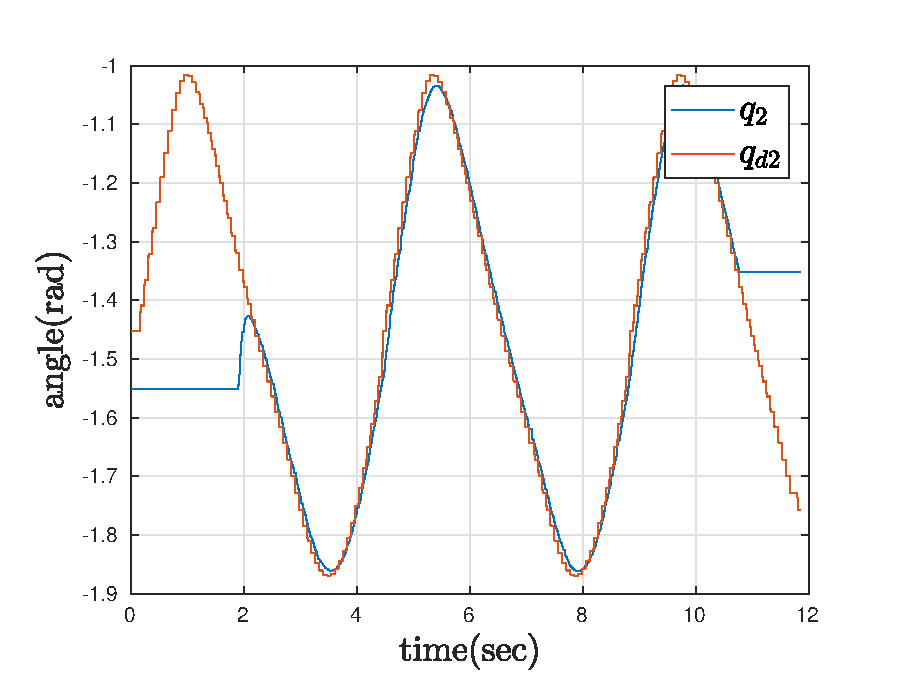
\includegraphics[width = \picsSiz\linewidth]{img/pathF2ff.eps}
        \caption{ }
    \end{subfigure}
    ~
    \centering
    \begin{subfigure}[htbp]{0.45\textwidth}
        \centering
        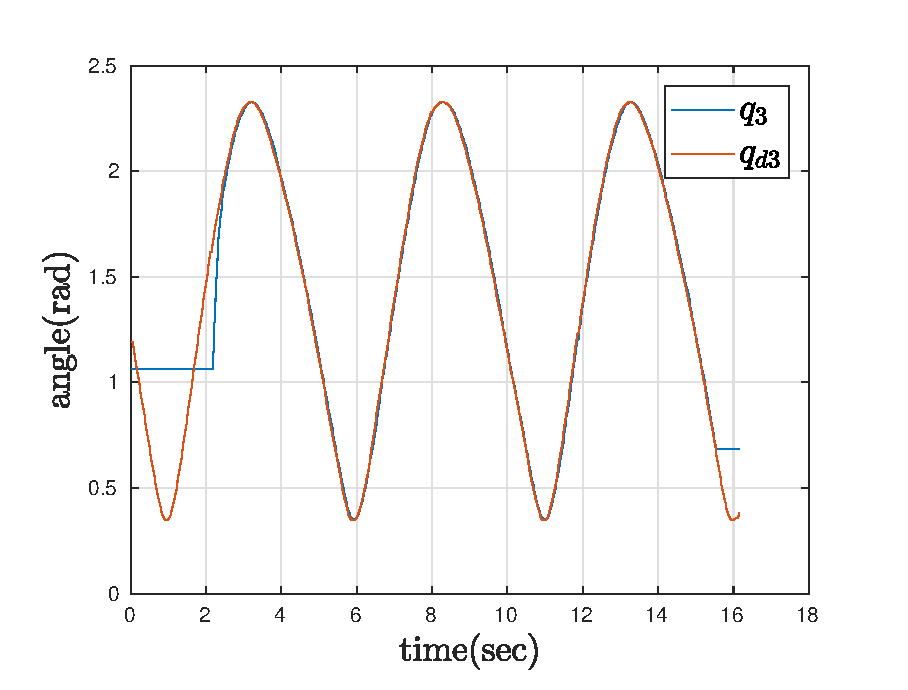
\includegraphics[width = \picsSiz\linewidth]{img/pathF3ff.eps}
        \caption{ }
    \end{subfigure}
    ~ 
    \begin{subfigure}[htbp]{0.45\textwidth}
        \centering
        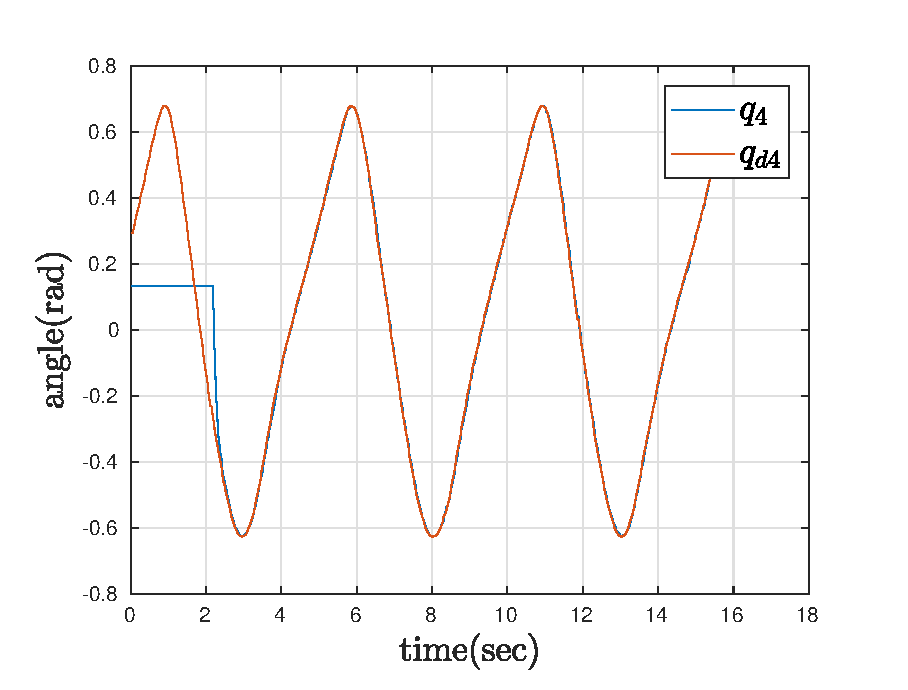
\includegraphics[width = \picsSiz\linewidth]{img/pathF4ff.eps}
        \caption{ }
    \end{subfigure}
    ~
    \begin{subfigure}[htbp]{0.45\textwidth}
        \centering
        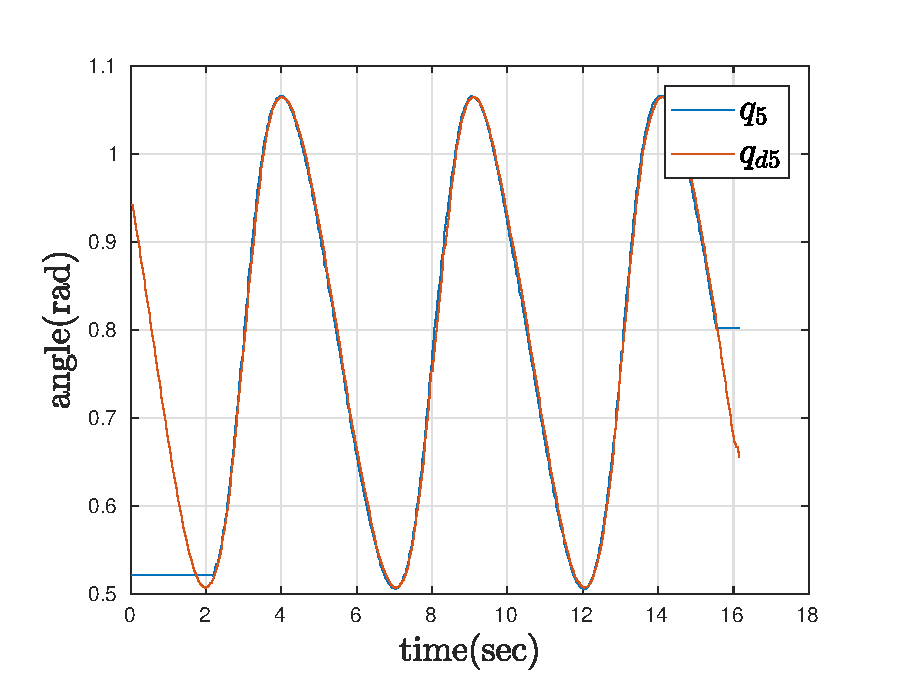
\includegraphics[width = \picsSiz\linewidth]{img/pathF5ff.eps}
        \caption{ }
    \end{subfigure}
    \caption{Path following with trajectory planner}
    \label{fig:pathTSff}
\end{figure*}
\newpage

\section{Motion planning}
Until now we have just used a predefined path that has been made to test the different aspects of the controller. If it is wanted to go from one point to another, it can be solved by creating a spline between these two points and do path following\cite{Spline,MatlabSpline2,MatlabSpline}. The task is not so easy if there are obstacles present. We then need to find the set-points such that the obstacle is avoided. One algorithm for solving this is the \textit{rapidly-exploring random tree (RRT)} which gives good results without any parameter tuning\cite{Lavalle}. 

\subsection{Rapidly exploring Random Tree (RRT)}
The RRT algorithm is creating a space-filling tree. In our case it can be used with obstacles in the search space such that the obstacle will be an illegal object where the three cannot expand. Then the shortest path is used to find a path trough the tree such that we get to the desired point and avoiding the obstacle. In \autoref{alg:rdt} one can see the \textit{simple rapidly exploring dense trees(RDT)} algorithm presented by \cite{Lavalle}. The difference between RRT and RDT is that the RDT is using a dense sequence $\alpha(i)$, and for RRT $\alpha(i)$ is a random value. This algorithm is without obstacle avoidance. If obstacle avoidance is wanted one have to check that the new edge does not intersect the obstacle. %If it intersects one have to find another vertex.\\\\
\begin{algorithm}[htbp]
 %\KwData{this text}
 %\KwResult{how to write algorithm with \LaTeX2e }
 SIMPLE\_RDT($q_0$)\;
 $\mathcal{G}.init(q_0)$\;
 \For{$i=1$ to $k$}{
  $\mathcal{G}.add\_vertex(\alpha(i))$\;
  $q_n\longleftarrow NEAREST(S(\mathcal{G}),\alpha(i))$\;
  $\mathcal{G}.add\_edge(q_n,\alpha(i))$\;
 }
 \caption{RDT algorithm}
 \label{alg:rdt}
\end{algorithm}

Reference \cite{rrt} provides code to find a path using RRT. In \figref{fig:rrt2dex} an example is given of the algorithm. An obstacle has been placed in the search space and the wanted point is behind the obstacle relative to the start point which in this case is the origin \cite{rrt}.
\begin{figure}[htbp]
  \centering
  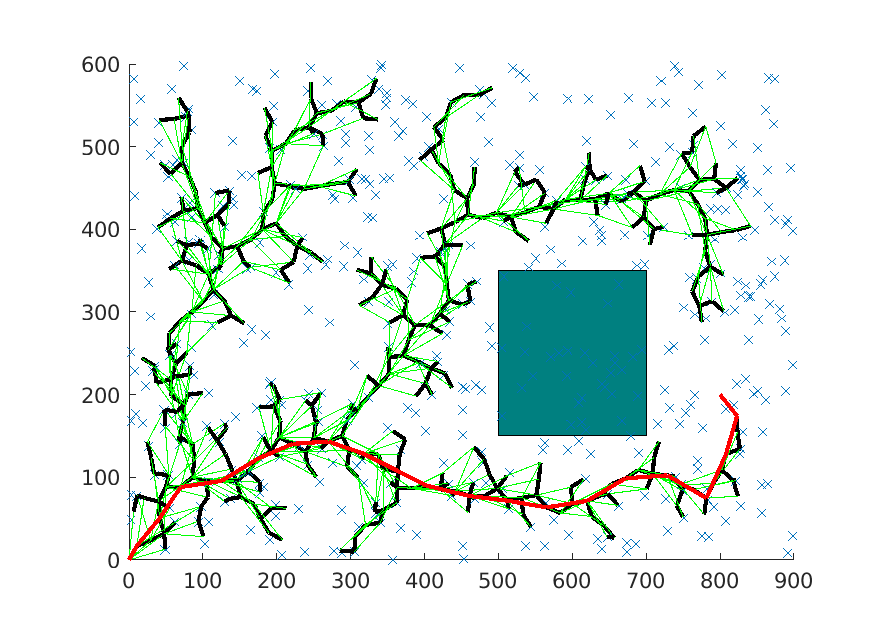
\includegraphics[width=.9\textwidth]{img/rrt2dex.eps}
  \caption{2D example of the RRT algoritm}
  \label{fig:rrt2dex}
\end{figure}

The next step is to expand this to a 3D example and do the same there. The code provided by \cite{rrt} does include 3D RRT, but not with obstacle avoidance unfortunately. But the source code is given, which mean it can be augmented into covering 3D obstacle avoidance. In \figref{fig:rrt3dex} the result of RRT in 3D space is presented. The red line is the lines between the nodes in the tree which shows a path to the desired point. 
\def\picsSiz{1.08}
\begin{figure*}[htbp]
    \centering
    \begin{subfigure}[htbp]{0.45\textwidth}
        \centering
        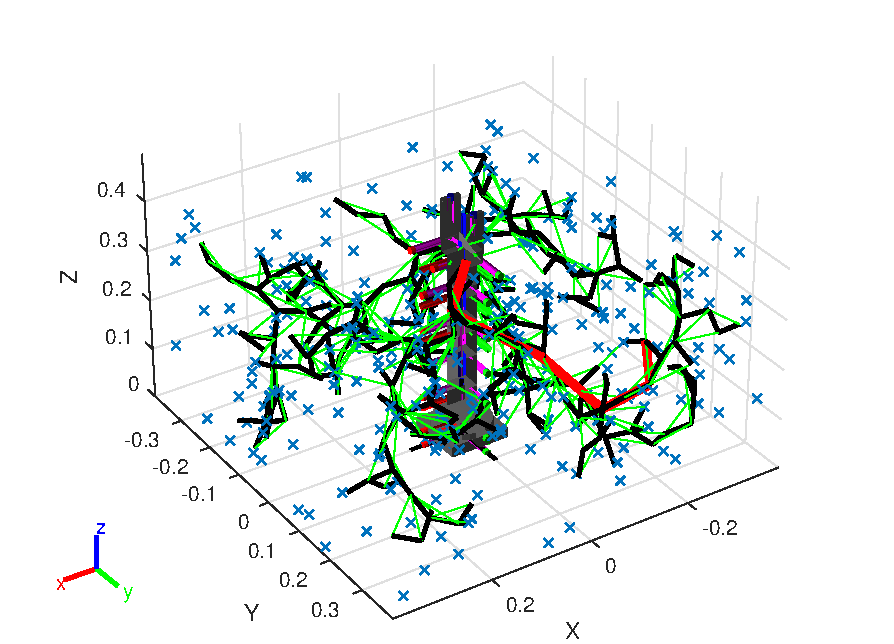
\includegraphics[width = \picsSiz\linewidth]{img/rrt3dex.eps}
        \caption{Result of the RRT algorithm}
        \label{fig:rrt3dex}
    \end{subfigure}
    ~ 
    \begin{subfigure}[htbp]{0.45\textwidth}
        \centering
        \includegraphics[width = \picsSiz\linewidth]{img/rrtSpline.eps}
        \caption{A spline is found based on the results}
        \label{fig:rrtSpline}
    \end{subfigure}
    \caption{3D example of the RRT algoritm}
    \label{fig:rrtsuper}
\end{figure*}
 As one can see in \figref{fig:rrt3dex} there are some green lines. These lines can be seen as shortcuts between each node the length of these shortcuts can be changed. In \figref{fig:rrtSpline} we have a path that is more complicated than it should be and one should maybe consider to increase the length of the shortcuts to get less nodes. This means that if the shortcut length is big enough the path will be a straight line from the desired point to the starting point of the tree. Given that the tree has found a path to the point. 
 
 \subsubsection{Obstacle avoidance}
 There is no point in doing the RRT if one does not have an obstacle to avoid. When an obstacle is added to the searchspace one have to check if the line connecting the new node to its parent node does not intersect with the object. The same has to be done with the shortcuts. To check if the edgdes and lines intersects with the obstacle Smits algorithm for ray intersection with a box is used\cite{Smits,Intersection}. In \figref{fig:obav} one can see the results when an obstacle is added into the workspace. The RRT algorithm finds as decent path and a spline is generated based on the results. 

\def\picsSiz{1.08}
\begin{figure*}[htbp]
    \centering
    \begin{subfigure}[htbp]{0.45\textwidth}
        \centering
        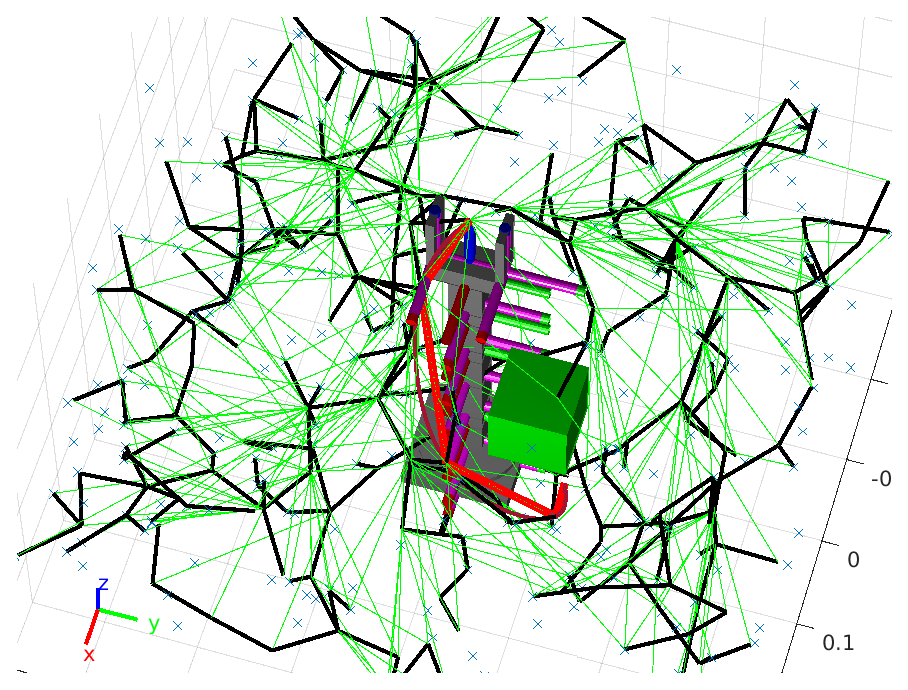
\includegraphics[width = \picsSiz\linewidth]{img/rrt3dOBav.eps}
        \caption{Result of the RRT algorithm with an obstacle}
        \label{fig:obav1}
    \end{subfigure}
    ~ 
    \begin{subfigure}[htbp]{0.45\textwidth}
        \centering
        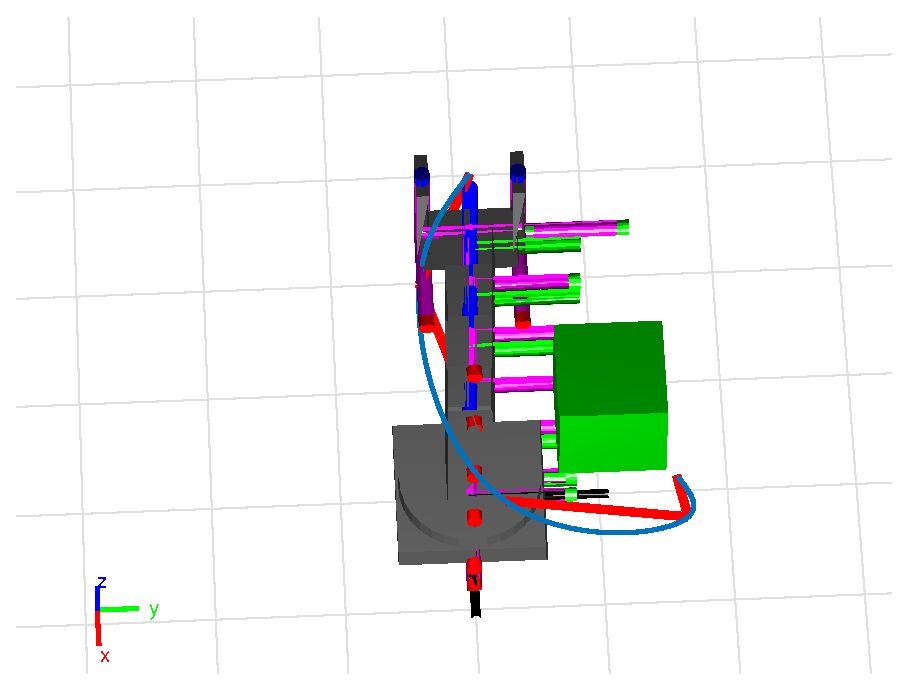
\includegraphics[width = \picsSiz\linewidth]{img/rrt3dOBavPath.eps}
        \caption{A spline is found based on the results}
        \label{fig:obav2}
    \end{subfigure}
    \caption{3D example of the RRT algoritm with obstacle present}
    \label{fig:obav}
\end{figure*}
